\newpage
\subsection{Caso d'uso UC4:  Login}
\label{UC4}
\begin{figure}[ht]
	\centering
	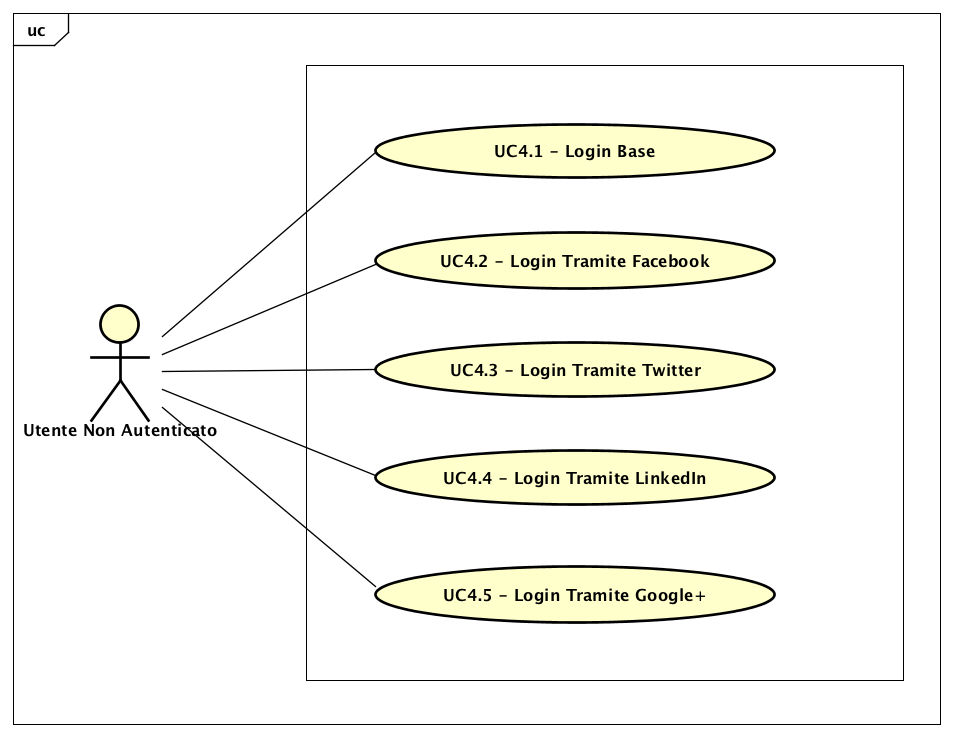
\includegraphics[scale=0.45]{UML/UC4.png}
	\caption{UC4: Login}
\end{figure}

\begin{longtable}{ l | p{11cm}}
	\hline
	\rowcolor{Gray}
	 \multicolumn{2}{c}{UC4 - Login}\\
	 \hline
	\textbf{Attori} & Utente Non Autenticato \\
	\textbf{Descrizione} & L'utente non autenticato inserisce le sue informazioni personali per potersi loggare all'applicazione web ed evolversi in un utente autenticato. Puo' effettuare login tramite Facebook, Twitter, LinkedIn, Google+ e tramite l'APIMarket stesso. \\
	\textbf{Pre-Condizioni} & L'utente ha scelto di loggarsi e l'applicazione web mostra la schermata di login \\
	\textbf{Post-Condizioni} & L'utente si è loggato all'applicazione web \\
	\textbf{Scenario Principale} & \begin{enumerate*}[label=(\arabic*.),itemjoin={\newline}]
		\item L'utente non autenticato può effettuare il login base (UC4.1)
		\item L'utente non autenticato può effettuare il login con Facebook (UC4.2)
		\item L'utente non autenticato può effettuare il login con Twitter (UC4.3)
		\item L'utente non autenticato può effettuare il login con LinkedIn (UC4.4)
		\item L'utente non autenticato può effettuare il login con Google+ (UC4.5)
	\end{enumerate*}\\
\end{longtable}